%f='selfrep'; b='selfrep'; pdflatex $f.tex && bibtex $f && pdflatex $f.tex && pdflatex $f.tex && rm $f.log $f.aux $b.bbl $b.blg && evince $f.pdf &>/dev/null &disown



\documentclass[12pt]{article}
\usepackage[margin=1in]{geometry}
\usepackage[protrusion=true,
            expansion=true]{microtype}
%\usepackage{amssymb}
%\usepackage{amsmath}
\usepackage{booktabs}
\usepackage{color}
\usepackage[usenames,
            dvipsnames]{xcolor}
\usepackage{graphicx}
\usepackage{caption}
\usepackage{subcaption}

\usepackage{kpfonts}
\usepackage[T1]{fontenc}
\usepackage{setspace}
\singlespacing
%\onehalfspacing
%\doublespacing

\newcommand{\term}[1]{\emph{#1}}

\begin{document}

\title{Programs that Program}

\author{Keenan Breik, Jason Liang}
\date{}
\maketitle

\begin{abstract}
\end{abstract}

\section{Introduction}
\label{intro}

Evolutionary computation allows computers
to automatically solve problems
that can be cast as optimization problems.
Until now, instantiations have been
in large part hand designed.
Designers struggle to find meaningful constructs
and optimal tunings.

We propose to allow computers
to automatically design such instantiations
by using evolutionary computation itself.
To do so, we desire programs
that write other programs
and thereby explore a search space.
In this paper,
we demonstrate that neural networks
can generate other meaningful neural networks.
[Be clear. Elaborate.]

%Section ? discusses related work.
%Section ? discusses decoding neural networks.
%Section ? discusses the evolutionary techniques used.
%Section ? discusses experiments with feedforward networks.
%Section ? discusses experiments with arbitrary networks.

The following is a quick overview of the rest of the paper: In section \ref{problemstatement}, we discuss the general problem of generating networks. In section \ref{feedforward}, we will go over methods for constructing self-replicating feed-forward neural networks. Next, in section \ref{results}, we will discuss experimental results. Finally in the last section, we present conclusions and future work.

\section{Decoding Networks}
\label{problemstatement}

A feedforward neural network $N$ encodes a function $f_N$
and thus is capable of storing information.
An arbitrary neural network $N$ encodes a program $P_N$
and thus is also capable of storing information.
One type of information a network may store
is an encoding of a second neural network $D(N)$.
But just as the meaning of a word
depends on the language being spoken,
so does the network encoded by $N$
depend on the semantics chosen.

To establish these semantics,
we may define what $N$ should be
in order to encode a given network $D(N)$.
This is the problem of \term{encoding}.
But if we want a network $N$
to generate another network $D(N)$,
then $D(N)$ is not given.
It is generated.
Solving the problem of encoding does not help.

An alternative way to establish the semantics
is to define what network $D(N)$ is encoded
by a given network $N$.
This is the problem of \term{decoding},
and we focus on it.
Solving the problem of decoding
consists of defining $D$
and allows us to have neural networks
generate other neural networks.

In order to give a network $N$
the power to generate another network
in an interesting way,
we prefer the decoding function $D$
to be neither completely stable
nor completely chaotic.
Instead, we want it somewhere around the edge of chaos.%
\cite{langton1990edgechaos}
This seems to pose a challenge,
but the function or program a neural network encodes
satisfies exactly this property.
So we can define $D(N)$ in terms of $f_N$ or $P_N$.
In other words, part of computing $D(N)$
can be applying $f_N$ or $P_N$.

We can consider the features of $D(N)$,
such as how its neurons connect,
to be stored at particular points
in $f_N$
or to be outputs of $P_N$.
%We query $N$ to extract the features of $D(N)$
%by applying $f_N$ or $P_N$ at particular points.
%In this way,
%we draw on the notion of a compositional
%pattern-producing network.\cite{stanley2007cppn}

\section{Self-Replicating Feed-forward Neural Networks}
\label{feedforward}

To create a self-replicating feed-forward neural network, we first use the pyBrain neural network library \cite{schaul2010} to create an initial neural network that has a fixed topology. By fixed topology, we mean that the number of input neurons, output neurons, hidden layers, neurons, and number of connections remain constant. The only parameters we plan to optimize in order to generate self-replicating neural networks are  the weights of the connections between neurons. Since a feed-forward neural network can have many variations in its topology, we have chosen a simple structure that makes the most sense. 

One major challenge is deciding what kind of input to feed into the neural network and how to interpret the output of the neural network as another neural net. For simplicity, we decided on giving our neural network a N-bit vector of binary numbers as input. If we topologically linearize all the connections in the neural network, we can associate the value of binary vector with a corresponding connection. For example, the binary vector 1001 can be associated with the 5th connection in a small network with 8 connections in total. Accordingly, the output of the neural network is a single value and it represents the weight of the connection specified by the input vector. Thus, by feeding the neural network a set of inputs that map to all the connections in the network, we can generate weights for each of connections. This means that the network is capable of generating another net exactly like itself in topology, but with possibly different connection weights. 

The next step is come up with a method to optimize the connection weights of the original network such that child network generated also has the same connection weight. Given the lack of gradients in this problem, we decide to rely on a black-box optimization approach to optimize the connection weights of the parent network. Thus we will require a fitness function that evaluates how close the the neural network is to generating a child network exactly like itself. To compute a fitness value, as seen in Fig.~\ref{pseudo}, we use the parent network to compute the connection weights of the child network, determine the error between the new connection weight and its original value in the parent network, and return the sum of all the errors. Now we can try a variety of different black-box optimization methods, including genetic algorithms \cite{deb2002fast}, CMAES \cite{hansen2003reducing}, and NES \cite{wierstra2008natural} to try to minimize the error and maximize the fitness of the neural network. Experimentally, we found that using CMAES resulted the most improvement in fitness every generation. 

\begin{figure}[h]
\begin{center}
  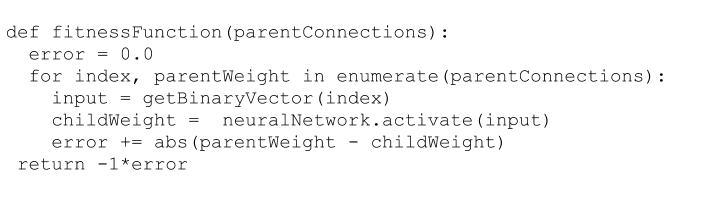
\includegraphics[width=0.8\linewidth]{pseudo.png}
\end{center}
   \caption{Function for computing fitness of a neural network. For each connection in the parent network, we convert it into a binary vector, feed it as input, and get the connection weight of the same connection in the child network. We compare the difference between the child and parent weights and sum up all differences as error, which is then inverted to become a fitness value.}
\label{pseudo}
\end{figure} 

\section*{Related Work}

Genetic programming?
Compositional pattern-producing networks.

%We consider ? schemes.
%[x0 ... xn] [y0 ... yn] ---> w
%[L S t s] ---> [n n w]
%arbitrary network

%\section{Evolution}
%algorithms. fitness functions.

\section{Experimental Results}
\label{results}

\section{Conclusion. Future Work.}
\label{conclusion}

\renewcommand{\refname}{\section{References}}
\bibliography{selfrep}
\bibliographystyle{plain}

\end{document}
